\chapter{Algorithm}
\label{ch:algorithm}

In this chapter the algorithm is discussed, presenting how the objects are recognized, and how the symbolic predicates are obtained. 

\section{Object Localization} 
For the planner, to know how to move the object, is fundamental knowing the objects on the scenario, therefore they need to be detected. More correctly, they need to be segmented since the algorithm is dealing with unknown objects, it is not going to recognize an objects as a particular one, but it segments the objects. 

This stage is composed on two steps:
\begin{enumerate}
\item Detecting the table top objects
\item Segmenting the table top objects
\end{enumerate}
The depth sensor is recording a depth map of a table, the algorithm has therefore to detect first the table, and so the objects that stands on top of it, and then segmenting them. We don't want to segment the entire image, if so, the table will be segmented as an object and the floor as well.

\subsection{Tabletop Object Detection} 
The strategy for the tabletop object detection phase is composed of 3 different steps:
\begin{enumerate}
\item \textbf{Table plane estimation} (by RANSAC): the points of the table are detected estimating first a plane in the point cloud, all the points which belong to such a plane are the points of the table. 
\item \textbf{2D Convex Hull of the table}: having the points of the table a 2D convex hull is computed in order to get a 2D shape containing those points.
\item \textbf{Polygonal prism projection}: all the points are projected on the table plane previously estimated and all the points which projections belong to the 2D convex hull are considered to be points of tabletop objects. 
\end{enumerate}

\begin{figure}[htp]
\centering
\begin{subfigure}[t]{0.32\textwidth}
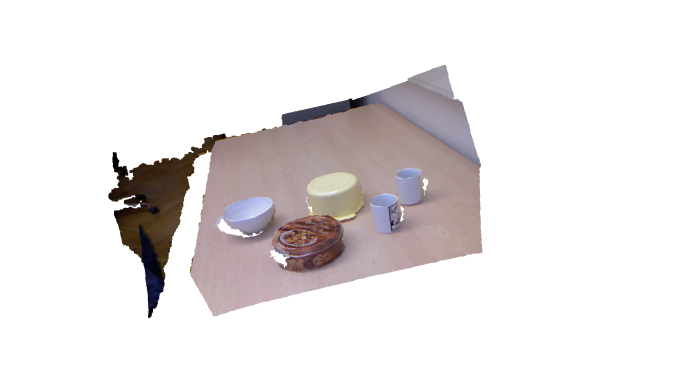
\includegraphics[width = 1.1\textwidth]{Img/ObjectSegmentation/pcl.png}
\caption{Input Point Cloud}\label{img:obj_pointcloud}
\end{subfigure}
\begin{subfigure}[t]{0.32\textwidth}
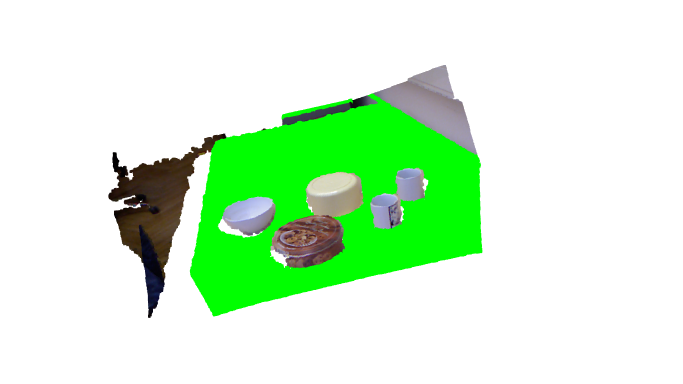
\includegraphics[width = 1.1\textwidth]{Img/ObjectSegmentation/ransac.png}
\caption{RANSAC plane estimation}\label{img:obj_ransac}
\end{subfigure}
\begin{subfigure}[t]{0.32\textwidth}
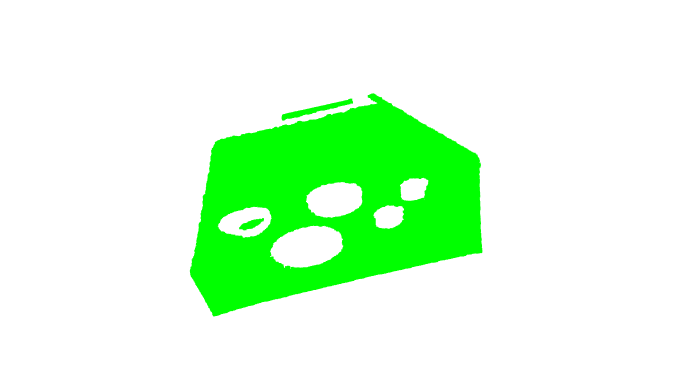
\includegraphics[width = 1.1\textwidth]{Img/ObjectSegmentation/plane.png}
\caption{Table plane}\label{img:obj_plane}
\end{subfigure}
\begin{subfigure}[t]{0.32\textwidth}
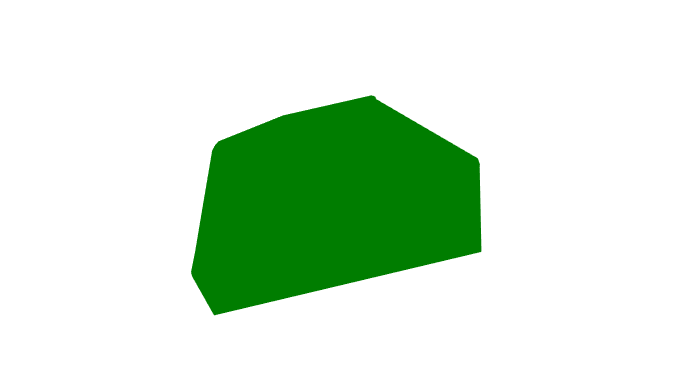
\includegraphics[width = 1.1\textwidth]{Img/ObjectSegmentation/convex_hull.png}
\caption{Convex Hull}\label{img:obj_conex_hull}
\end{subfigure}
\begin{subfigure}[t]{0.32\textwidth}
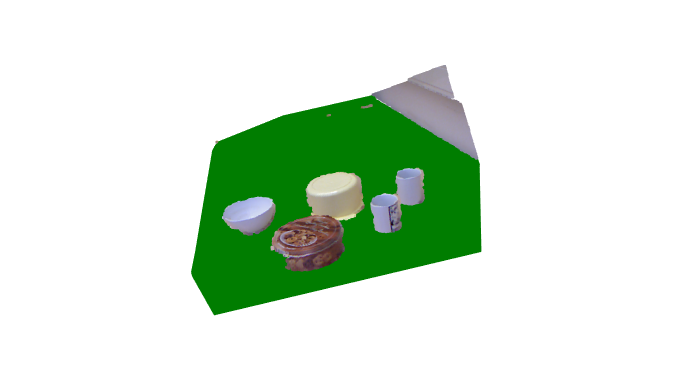
\includegraphics[width = 1.1\textwidth]{Img/ObjectSegmentation/convex_hull_full.png}
\caption{Convex hull in the point cloud}\label{img:obj_convex_hull_full}
\end{subfigure}
\begin{subfigure}[t]{0.32\textwidth}
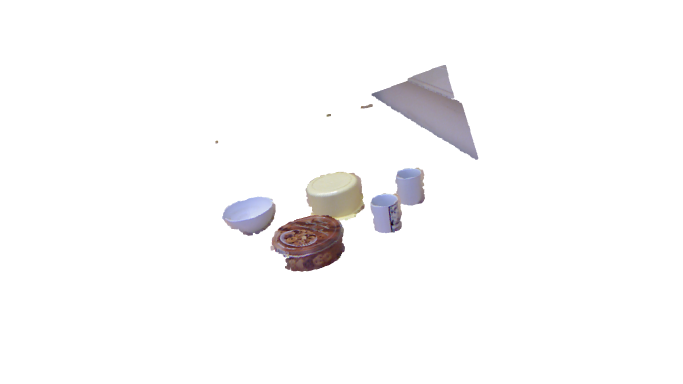
\includegraphics[width = 1.1\textwidth]{Img/ObjectSegmentation/tabletop_objects.png}
\caption{Tabletop objects}\label{img:obj_tabletop_objects_results}
\end{subfigure}
\caption{\textbf{Object Segmentation:} Given the point cloud (\subref{img:obj_pointcloud}), the estimated table's plane is obtained (\subref{img:obj_ransac} and \subref{img:obj_plane}), its convex hull is extracted (\subref{img:obj_conex_hull} and \subref{img:obj_convex_hull_full}), and the tabletop objects are obtained by a polygonal prism projection (\subref{img:obj_tabletop_objects_results}).}
\label{img:obj_tabletop_objects}
\end{figure}

The steps of this tabletop object detection algorithm are described in Figure \ref{img:obj_tabletop_objects}   for the point cloud\footnote{Point cloud taken from the Object Segmentation Database (OSD) \href{http://users.acin.tuwien.ac.at/arichtsfeld/?site=4}{http://users.acin.tuwien.ac.at/arichtsfeld/?site=4}} in Figure \ref{img:obj_pointcloud}.

\subsection{Object Segmentation}
\label{sec:obj_seg}
Once the objects on the table are detected the following phase is to segment them in order to get a point cloud per object.

\subsubsection{Supervoxel}

For their segmentation the supervoxel concept is used. A supervoxel is a group of voxels that share similar characteristics. 
%and it is equivalent to the superpixel concept for the voxel case. Superpixel is a widely used preprocessing step in segmentation
%algorithms  which allows to reduce the number of regions
%that must be considered later by more computationally
%expensive algorithms, with a minimal loss of information. 
%The supervoxel concept is the extension of the superpixel method to the point clouds. A voxel represents a single sample on a regularly spaced, three-dimensional grid. A supervoxel 

In this work the supervoxels are computed with the Voxel Cloud Connectivy Segmentation (\texttt{VCCS}) algorithm \cite{Papon13CVPR}, which was proposed in 2014 and gives good improvements with respect to previous state of the art methods, and still it is able to be used in online applications. 

The algorithm works in 4 main steps:
\begin{itemize}
\item Voxelizing the point cloud
\item Creating an adjacency graph for the voxel-cloud 
\item Creating seeds for the initial supervoxels centres
\item Each seed is described by $39$ features that describe spatial coordinates, colors and local surface model properties. Then a distance metric based on  these features is defined. 
\item Clustering the voxels into supervoxles iteratively by means of the distance metric, the adjacency graph, and the search volume of the supervoxel. 
\item Once the search of all supervoxel adjacency graphs has been concluded, the centres of each supervoxel is updated by taking the mean of all its constituents. 
\end{itemize} 

\subsubsection{Local Convex Connected Patches Segmentation}
\label{sec:LCCP}
Once the supervoxels of the objects are computed, they can be clustered in order to segment the objects. Papon et al. also proposed a segmentation algorithm based on their supervoxel technique, called \textit{Local Convex Connected Patches Segmentation} (\texttt{LCCP}) \citep{LCCP}. This algorithm permits to segment objects by clustering together adjacent convex supervoxels.  The algorithm is quite simple but very good for segmentation of objects that have convex shapes, in Figure \ref{img:LCCP_structure} the algorithm is briefly described. 

\begin{figure}[h]
\centering
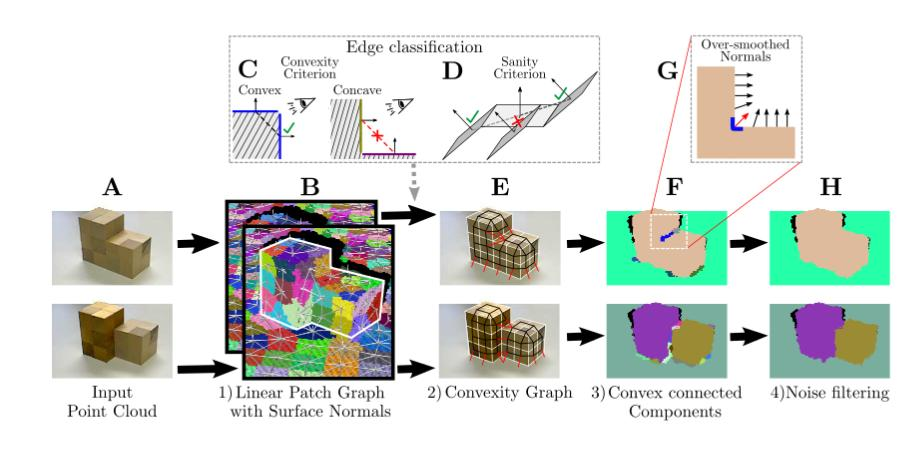
\includegraphics[width=\textwidth]{Img/ObjectSegmentation/lccp_structure.jpg}
\caption{\texttt{LCCP} algorithm's structure. Reproduced from \citep{LCCP}}
\label{img:LCCP_structure}
\end{figure}

It clusters all the adjacent convex supervoxels (patches) using two criterion:
\begin{itemize}
\item Extended criterion: to consider two adjacent patches convex, both must have a connection to a patch which is convex with respect both patches
\item Sanity Criterion: check if the adjacent patches which can be considered as convex present geometric discontinuities (see point D of Figure \ref{img:LCCP_structure}), in this case they are not considered as valid to form a cluster.
\end{itemize}
Then, due to the smoothed normals that could appear in some edges of the objects (point G Figure \ref{img:LCCP_structure}), the algorithm merges the clusters that are composed of few supervoxels to the biggest adjacent cluster. 

By tuning properly the parameters of the segmentation algorithm the objects can be correctly segmented obtaining for one of them a point cloud. Two examples of the segmentation algorithm for a cluttered scene are depicted in Figure \ref{fig:seg_results}. 

\begin{figure}[h]
\centering
\begin{subfigure}[t]{0.2\textwidth}
\centering
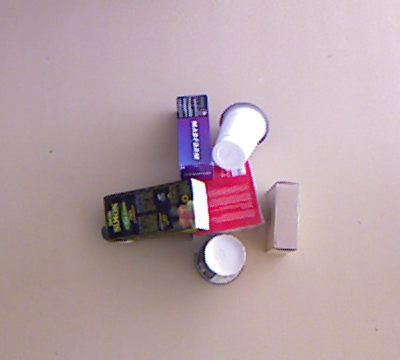
\includegraphics[width=\textwidth]{Img/ObjectSegmentation/seg1_rgb.png}
\end{subfigure}
\begin{subfigure}[t]{0.2\textwidth}
\centering

\includegraphics[width=\textwidth]{Img/ObjectSegmentation/seg1.png}
\end{subfigure}
\hspace{1.5cm}
\begin{subfigure}[t]{0.2\textwidth}
\centering
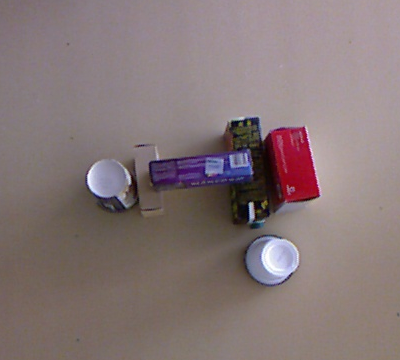
\includegraphics[width=\textwidth]{Img/ObjectSegmentation/seg2_rgb.png}
\end{subfigure}
\begin{subfigure}[t]{0.2\textwidth}
\centering
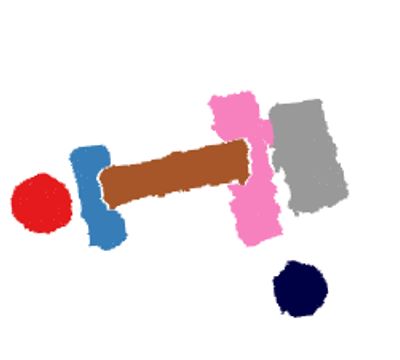
\includegraphics[width=\textwidth]{Img/ObjectSegmentation/seg2.png}
\end{subfigure}
\caption{Example of segmentation results.}\label{fig:seg_results}
\end{figure}

Note that the algorithm works mainly considering geometric properties, and not the color of the pixels. Considering the colors could lead to worst segmentation results for our case of studio since many objects have no only one color.

\begin{wrapfigure}{r}{6.5cm}
\centering
\caption{Box with a green stripe.}\label{fig:seg_color}
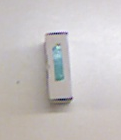
\includegraphics[width=3.5cm]{Img/ObjectSegmentation/color_seg_problem.png}
\end{wrapfigure}
A color based segmentation could segment a draw, or a small part of the object, as a different object, but this, accordingly to the strategy we are going to use (see next sections), would lead to an unfeasible problem. 
For instance, in Figure \ref{fig:seg_color} is shown a box with a green stripe on its top surface, a segmentation algorithm based also on colors could lead to segment the green stripe as another object, and the result is that it is impossible to grasp the green stripe without collide with the box. Vice versa, any interaction with the box is impossible without having a collision with the green stripe. This is the main reason the segmentation we used is based only on geometric features (The \ttt{LCCP} algorithm has the option to include color importance but we neglected it). 


\section{Background}
%\begin{itemize}
%\item collison detection
%\item pca
%\item table projection - convex hulls
%\item rotation matrices
%\end{itemize}

In this section will be presented some concepts that will be used to execute the actions and to compute the predicates. 

\paragraph{Principal Components}
The first concept to know is the concept of principal directions. The principal direction of an object is its principal axis which is defined as any of three mutually perpendicular axes about which the moment of inertia of a body is maximum. For instance, for a rectangular object its principal direction is the axis aligned with its longest dimension. 

To obtain the principal axis the principal component analysis (PCA) \citep{PCA} technique is used. This technique is a common statistical procedure that uses orthogonal transformation to convert a set of  observations of possibly correlated variables into a set of values of linearly uncorrelated variables, which are called principal components. The transformation is defined in a manner that the first component has the largest variance, the second has the second largest variance and so on. The principal components are orthogonal because they are the eigenvectors of the covariance matrix, which is symmetric. An example of the principal components for a 2D data set is depicted in Figure \ref{fig:pca1}\footnote{Image taken from \href{https://en.wikipedia.org/wiki/Principal_component_analysis}{https://en.wikipedia.org/wiki/Principal\_component\_analysis}}. The principal components are computed through the covariance matrix of the set of observation, and its eigenvectors $\bar{\lambda_v}$ represent the principal components while its eigenvalues $\lambda$ represent the variance of the data set along the principal component $\bar{\lambda_v}$. 

\begin{figure}[h]
\centering
\begin{subfigure}[t]{0.45\textwidth}
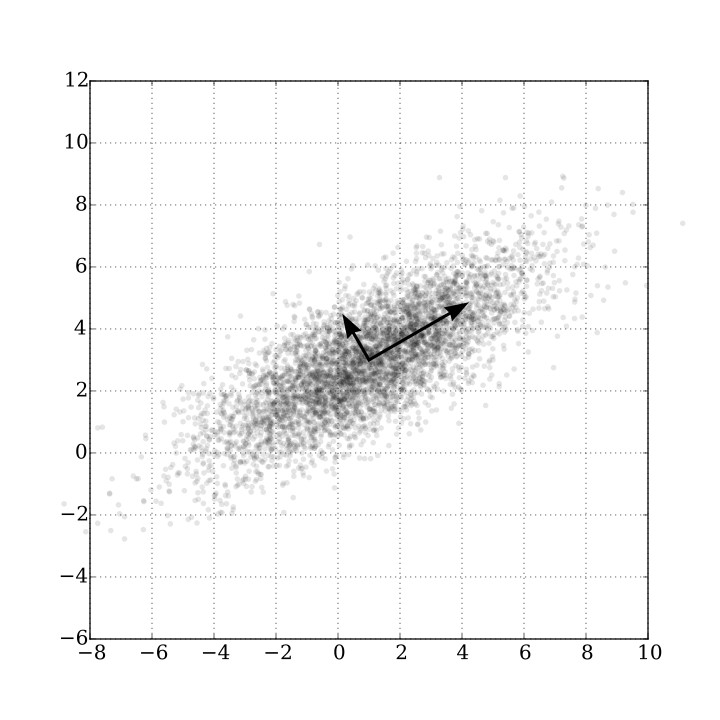
\includegraphics[width=\textwidth]{Img/pca/pca.png}
\caption{}\label{fig:pca1}
\end{subfigure}
\begin{subfigure}[t]{0.45\textwidth}
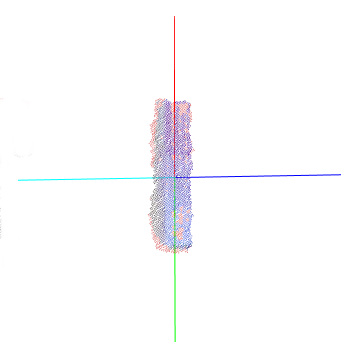
\includegraphics[width=\textwidth]{Img/pca/pca2.png}
\caption{}\label{fig:pca2}
\end{subfigure}
\caption{\textbf{Principal Components Analysis -} In Figure \ref{fig:pca1} PCA for a standard 2D set of observations. In Figure \ref{fig:pca2} results of the PCA for a rectangular segmented object. The \textcolor{green}{green}, \textcolor{red}{red} lines refers to different ways of the first principal components, while \textcolor{blue}{blue} and \textcolor{cyan}{cyan} lines refers to different ways of the second principal directions. The third one would be orthogonal to the first two principal components.}
\end{figure}

A generic point cloud can be seen as a set of observations and the PCA can be directly applied in to the object's point cloud to retrieve its principal components, or how called in this work principal directions. In Figure \ref{fig:pca2} the principal directions of a generic object are illustrated. 

\paragraph{Projection onto a plane}
We will see later that several things need the concept of the projections of a point into a plane. Considering a point $p={x_p,y_p,z_p}$ and a plane $P$ defined by the following equation
\begin{equation}
a x + by + cz + d = 0
\end{equation}
the projection $p_P$ of point $p$ onto the plane $P$ is given by the following set of operations:
\begin{enumerate}
\item Given the origin point $P_0=(x_0,y_0,z_0)$ of the plane, which can be calculated by arbitrary $x_0$ and $y_0$ coordinates as
\[
z_0 = \frac{-1}{c}(ax_0 + by_0 + d),
\]
\item calculate the coordinates of $P_0$ with respect the point $p$
\[
P^{p} = p - P_0,
\]
\item then calculate its projection $\lambda_p$ onto the plane normal $n=(a,b,c)$
\[
\lambda_p = \bar{n} \cdot p^{plane}, 
\]
\item compute the coordinates of the projection onto the plane of point $p$ with respect to the point itself:
\[
p_P^p = - \lambda_p \bar{n}
\]
\item translate it by the coordinate of the points in order to have the projection of the point expressed with respect the original reference frame:
\[
p_P = \bar{p_P}^p + p. 
\]
\end{enumerate}

\paragraph{Rotation Matrices}
Rotation matrices are matrices which express a rotation between two reference frames. Given two frames $\{A\}$ and $\{B\}$, and the rotation matrix $\prescript{A}{B}R$ that defines the rotation of $\{B\}$ relative to $\{A\}$ then a point $\prescript{A}{}P$ with respect frame $\{A\}$ is given by $\prescript{A}{}P=R^{A}_{B}\prescript{B}{}P$, where $\prescript{B}{}P$ is the same point relative frame $\{B\}$. 

Having a desired frame $\{B\}$ defined by axis $\hat{\prescript{A}{}X_B},\hat{\prescript{A}{}Y_B}$ and $\hat{\prescript{A}{}Z_B}B$, where $\hat{\prescript{A}{}Y_B}$ is the y axis of frame $\{B\}$ relative to frame $\{A\}$, the rotation matrix between $\{B\}$ and $\{A\}$ is defined as
\[
R^{A}_{B} = 
\begin{bmatrix}
\hat{\prescript{A}{}X_B} \\
\hat{\prescript{A}{}Y_B} \\
\hat{\prescript{A}{}Z_B} \\
\end{bmatrix}
\]
To transform any object, such as the gripper mesh model, to frame $\{B\}$ then the following homogeneous transform is applied:
\[
H = 
\begin{bmatrix}
R^{B}_{A} & \prescript{A}{}B_O \\
\bar{0} & 1
\end{bmatrix}
\]
where  $R^{B}_{A}={R^{A}_{B}}^{\top}$ and $\prescript{A}{}B_O$ is the origin of frame $\{B\}$ relative to $\{A\}$. In this way, having some axis that defined our new reference frame, we can transform the gripper model in such a way its closing point is in the origin of the new frame and its orientation is the one defined by the new reference frame. 

\paragraph{Convex Hull}
A convex hull of a point cloud $P$ is the smallest 3D convex set that contains $P$. 
\begin{figure}[h]
\centering
\begin{subfigure}[t]{0.3\textwidth}
\centering
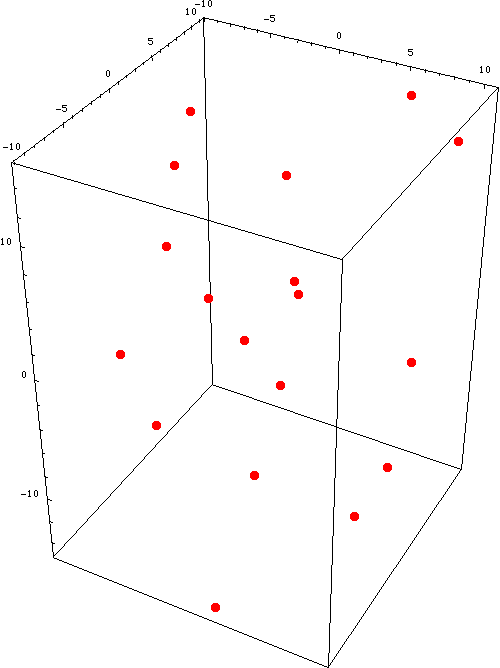
\includegraphics[height=4cm]{Img/convexhull/ch1.png}
\caption{Pointcloud}
\end{subfigure}
\begin{subfigure}[t]{0.3\textwidth}
\centering
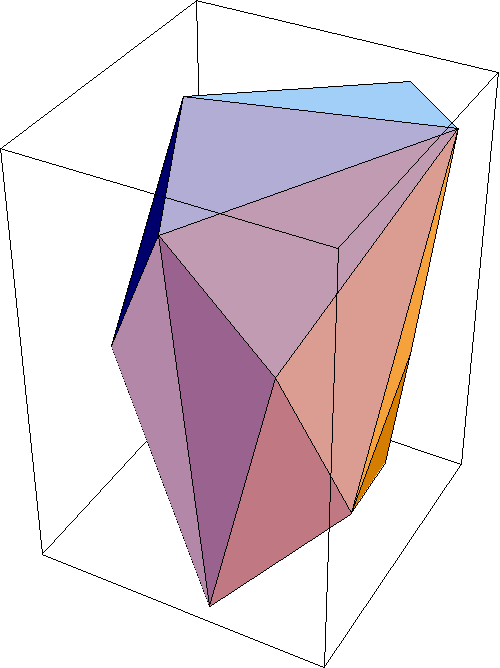
\includegraphics[height=4cm]{Img/convexhull/ch3.png}
\caption{Convex hull}
\end{subfigure}
\caption{Convex hull example}\label{fig:convexhull_example}
\end{figure}
In Figure \ref{fig:convexhull_example} an example of the convex hull for a point cloud is shown. The vertices are first detected and then connected among them by means of triangles. In this way a triangle mesh is associated to the convex hull. 

\paragraph{Collision Detection}
To understand if an object impeds a certain action, such as the pushing along a direction, we have to check if along the desired trajectory the pushed object will collide with a certain one. The collision detection is therefore a crucial step for the predicates computation. There exist different techniques to assert if two objects are colliding, all of them need a representation of the object, which could be for example a basic shape or a more complex as an octree. 

The mesh shape has been thought to use since it can be directly obtained from a \textit{convex hull}. 

Given two objects A and B and their configurations $\bf{q_A}$ and $\bf{q_B}$, the discrete collision query returns a boolean value about whether two objects collide or not. Two objects collide if
\[
A(\bf{q_A}) \cap B(\bf{q_B}) \neq 0
\]

The collision detection will be used to understand if in a given pose $\bf{q}$ the object $A$ will collide with the other objects in the scene.

\paragraph{Objects Modelling}
The triangle mesh needed for the collision checking can be directly retrieved by the convex hull. But there is a consideration to take into account. The Kinect, given its pose, is only able to see mainly the top surface of the objects and not all the sides, and therefore we cannot apply directly the convex hull algorithm to the detected surfaces. If we would apply the convex hull on an object's surfaces, we will have likely the situation in which a surface $S$ transformed in a configuration such that it will be above or below another one, and the collision detection will detect no collision since the two surfaces are not colliding. This is because we are totally missing the rest of information about the geometry of the object since we only know the objects surfaces.

\begin{figure}[h]
\centering
\begin{subfigure}[t]{0.45\textwidth}
\centering
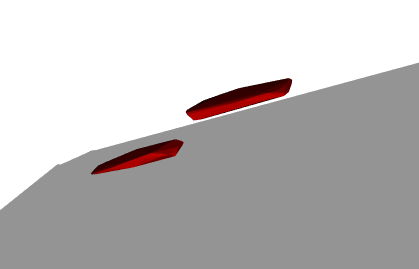
\includegraphics[width=\textwidth]{Img/convexhull/cv_top.png}
\caption{}\label{fig:cv_top}
\end{subfigure}
\begin{subfigure}[t]{0.45\textwidth}
\centering
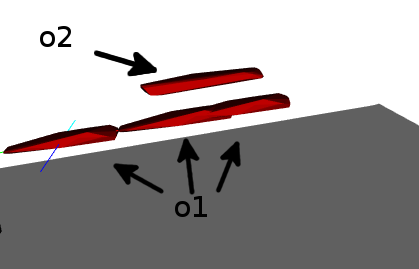
\includegraphics[width=\textwidth]{Img/convexhull/cv_top_collision.png}
\caption{}\label{fig:cv_top_collision}
\end{subfigure}
\caption{Convex hulls and collision detection using the segmented objects retrieved by the \ttt{LCCP} segmentation algorithm. The gray surface represents the plane's 2D convex hull. In Figure \ref{fig:cv_top} it is possible appreciating that we miss the information about the hidden part of the object. In Figure \ref{fig:cv_top_collision} a collision detection example is depicted. The convex hull is translated along a direction and no collision is detected with any possible translation since the two convex hull will not intersect.}
\end{figure}

From the Kinect's point cloud also the table plane is known, so all the information we have are:
\begin{itemize}
\item Table plane
\item segmented objects (mainly the top surfaces)
\end{itemize}
If an human would be in the same pose of the Kinect, looking at the table, it will imagine that the objects are not floating surfaces, and he/she will deduce the objects shape from the shape of the top surface. Since in this work we assumed to work with parallelepipeds, the sides of the objects can be easily deduced by projecting the top surface's edges to the plane and then filling the missing object's sides with points. To do that we have to detect the top surface's edges. A more trivial method is directly projecting all the points of the surfaces onto the table plane and then apply the convex hull algorithm the resulting point cloud given by the sum of the top surface and the projected one. In this way the missing sides are indirectly retrieved by the convex hull. 

%The PCL convex hull algorithm returns the convex hull as a triangular mesh, which can be used by the FCL for the collision detection. 

%The pose of the Kinect camera is above the table pointing forward it. In such a pose the Kinect is only able to see mainly the top side of the objects, and not their sides. 
%--- discussed the convex hull relating into to the neccesity for the collision detection.

\textbf{Somewhere talk about the limitation of the segmentation that is we assume it to be perfect because if not the planner will return likely an infeasible plan}

\section{Actions}

\subsection{Pushing}

Note that we can obtain with this method is:
\begin{itemize}
\item pushing direction for simple objects: we can push the rectangular object of Figure \ref{fig:pca2} along one of the ways of the first two principal directions, 
\item assign a reference frame to the object: by using the three principal components we can obtain a new reference frame $F_{o_i}$ for each object.
\end{itemize}

The computed principal components are orthogonal between themselves but the way of eigenvector $\bar{\lambda}$ is chosen by the PCA algorithm. In our case we are interested having a coherent description of the pushing directions as indicated in Figure \ref{fig:pca2}, and for that aim $\bar{\lambda_2}$ has to be always the same way with respect to the first principal component $\bar{\lambda_1}$. 

The reference frame --- AABB

\subsection{Grasping}

\section{Predicates Computations}
In Chapter \ref{ch:task_planner}  the predicates used are described, in this section their computation is presented in detail. 

Once the objects have been segmented, we have one point cloud per object, next we have to retrieve the symbolic predicates from the objects configuration. 

Before going in detail on their computation some general concepts useful to understand the algorithm are first presented. 

\subsection{Predicate: \texttt{block\_grasp}}
\subsection{Predicate: \texttt{on}}
\subsection{Predicate: \texttt{block\_dir$_i$}}
